\documentclass[tikz,border=14pt]{standalone}
\usepackage[no-math]{fontspec}
\usepackage{xeCJK}
\usepackage[UTF8,fontset=none]{ctex}
\usepackage{tikz}
\usetikzlibrary{arrows.meta,positioning,fit,calc,backgrounds,decorations.pathreplacing}

\IfFontExistsTF{Times New Roman}{\setmainfont{Times New Roman}}{\setmainfont{TeX Gyre Termes}}
\IfFontExistsTF{Kaiti TC}{\setCJKmainfont[AutoFakeBold=3]{Kaiti TC}}
  {\IfFontExistsTF{Songti TC}{\setCJKmainfont[AutoFakeBold=3]{Songti TC}}
    {\setCJKmainfont{PingFang TC}}}
% thesis_colors.tex ─ 論文統一 TikZ 色票定義
% 在每個 standalone 圖的 preamble 以 % thesis_colors.tex ─ 論文統一 TikZ 色票定義
% 在每個 standalone 圖的 preamble 以 % thesis_colors.tex ─ 論文統一 TikZ 色票定義
% 在每個 standalone 圖的 preamble 以 \input{thesis_colors.tex} 引入

\definecolor{thesisBlue}{RGB}{43,108,176}      % 訓練集、主箭頭、主色
\definecolor{thesisAmber}{RGB}{201,140,30}     % 驗證集、次要強調
\definecolor{thesisCrimson}{RGB}{155,35,53}    % 測試集、警示
\definecolor{thesisTeal}{RGB}{74,157,143}      % 節點類型 1（電子零組件）
\definecolor{thesisForest}{RGB}{45,122,79}     % 節點類型 2（光電及I/O）、LSTM Update
\definecolor{thesisSand}{RGB}{194,168,120}     % 節點類型 3（半導體）
\definecolor{thesisDark}{RGB}{45,55,72}        % 框線、文字、主箭頭
\definecolor{thesisLight}{RGB}{237,242,247}    % 淡背景、節點填色
\definecolor{thesisPurple}{RGB}{107,70,193}    % GAT 第二注意力頭
\definecolor{thesisMidGray}{RGB}{130,145,160}  % 次要線段、虛線
 引入

\definecolor{thesisBlue}{RGB}{43,108,176}      % 訓練集、主箭頭、主色
\definecolor{thesisAmber}{RGB}{201,140,30}     % 驗證集、次要強調
\definecolor{thesisCrimson}{RGB}{155,35,53}    % 測試集、警示
\definecolor{thesisTeal}{RGB}{74,157,143}      % 節點類型 1（電子零組件）
\definecolor{thesisForest}{RGB}{45,122,79}     % 節點類型 2（光電及I/O）、LSTM Update
\definecolor{thesisSand}{RGB}{194,168,120}     % 節點類型 3（半導體）
\definecolor{thesisDark}{RGB}{45,55,72}        % 框線、文字、主箭頭
\definecolor{thesisLight}{RGB}{237,242,247}    % 淡背景、節點填色
\definecolor{thesisPurple}{RGB}{107,70,193}    % GAT 第二注意力頭
\definecolor{thesisMidGray}{RGB}{130,145,160}  % 次要線段、虛線
 引入

\definecolor{thesisBlue}{RGB}{43,108,176}      % 訓練集、主箭頭、主色
\definecolor{thesisAmber}{RGB}{201,140,30}     % 驗證集、次要強調
\definecolor{thesisCrimson}{RGB}{155,35,53}    % 測試集、警示
\definecolor{thesisTeal}{RGB}{74,157,143}      % 節點類型 1（電子零組件）
\definecolor{thesisForest}{RGB}{45,122,79}     % 節點類型 2（光電及I/O）、LSTM Update
\definecolor{thesisSand}{RGB}{194,168,120}     % 節點類型 3（半導體）
\definecolor{thesisDark}{RGB}{45,55,72}        % 框線、文字、主箭頭
\definecolor{thesisLight}{RGB}{237,242,247}    % 淡背景、節點填色
\definecolor{thesisPurple}{RGB}{107,70,193}    % GAT 第二注意力頭
\definecolor{thesisMidGray}{RGB}{130,145,160}  % 次要線段、虛線


\begin{document}
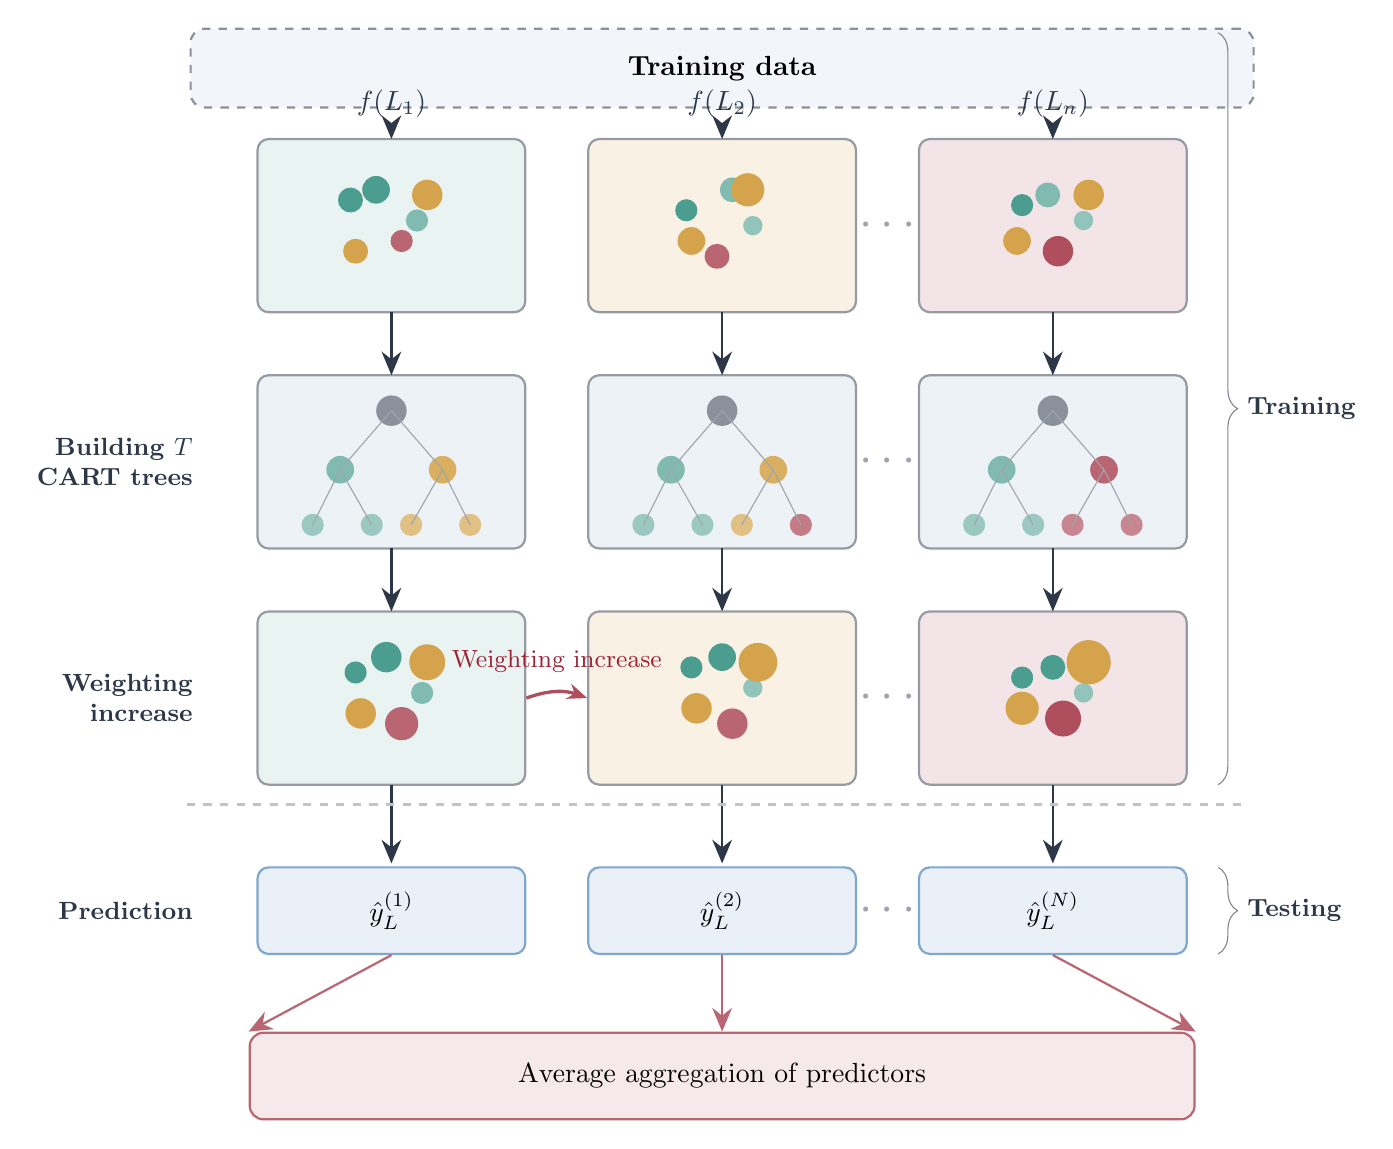
\begin{tikzpicture}[
  databox/.style={draw=thesisDark!50, fill=#1!12, rounded corners=4pt,
                  minimum width=3.4cm, minimum height=2.2cm, thick},
  treebox/.style={draw=thesisDark!50, fill=thesisLight, rounded corners=4pt,
                  minimum width=3.4cm, minimum height=2.2cm, thick},
  predbox/.style={draw=thesisBlue!60, fill=thesisBlue!10, rounded corners=4pt,
                  minimum width=3.4cm, minimum height=1.1cm, thick, align=center,
                  font=\normalsize},
  aggrbox/.style={draw=thesisCrimson!70, fill=thesisCrimson!10, rounded corners=5pt,
                  minimum width=12.0cm, minimum height=1.1cm, thick, align=center,
                  font=\normalsize},
  arr/.style={-{Stealth[length=3mm,width=2.5mm]}, thick, thesisDark},
  redarr/.style={-{Stealth[length=2.5mm,width=2mm]}, thick, thesisCrimson!80, line width=1.2pt},
  rowlabel/.style={font=\small\bfseries, thesisDark, align=right},
  coltitle/.style={font=\normalsize, thesisDark, align=center},
]

%% ── column x-centres ─────────────────────────────────────
\def\cx{0}     % L_1
\def\cy{4.2}   % L_2
\def\cz{8.4}   % L_n

%% ── row y-centres ────────────────────────────────────────
\def\ydata{7.5}    % scatter data row
\def\ytree{4.5}    % CART tree row
\def\yrdata{1.5}   % reweighted data row
\def\ypred{-1.2}   % prediction row
\def\yaggr{-3.3}   % aggregation row

%%──────────────────────────────────────────────────────────
%% TRAINING DATA HEADER
%%──────────────────────────────────────────────────────────
\node[draw=thesisDark!55, dashed, fill=thesisBlue!6, rounded corners=5pt,
      minimum width=13.5cm, minimum height=1.0cm, thick,
      font=\normalsize\bfseries] (hdr)
     at ({(\cx+\cz)/2}, 9.5) {Training data};

%%──────────────────────────────────────────────────────────
%% COLUMN 1  ( L_1 )
%%──────────────────────────────────────────────────────────
% --- scatter data
\node[databox=thesisTeal] (d1) at (\cx, \ydata) {};
\begin{scope}[shift={(\cx, \ydata)}]
  \foreach \px/\py/\pc/\ps in
    {-0.8/0.5/thesisTeal/4.5pt, -0.3/0.7/thesisTeal/5pt,
     0.5/0.1/thesisTeal!70/4pt, 0.7/0.6/thesisAmber!80/5.5pt,
     -0.7/-0.5/thesisAmber!80/4.5pt, 0.2/-0.3/thesisCrimson!70/4pt}{
    \fill[\pc] (\px*0.65, \py*0.65) circle(\ps);
  }
\end{scope}
\node[coltitle, above=4pt] at (d1.north) {$f(L_1)$};

% --- CART tree
\node[treebox] (t1) at (\cx, \ytree) {};
\begin{scope}[shift={(\cx,\ytree)}]
  \fill[thesisDark!55]   (0, 0.65) circle(5.5pt);
  \fill[thesisTeal!70]   (-0.65,-0.10) circle(5pt);
  \fill[thesisAmber!70]  ( 0.65,-0.10) circle(5pt);
  \fill[thesisTeal!55]   (-1.0,-0.80) circle(4pt);
  \fill[thesisTeal!55]   (-0.25,-0.80) circle(4pt);
  \fill[thesisAmber!55]  ( 0.25,-0.80) circle(4pt);
  \fill[thesisAmber!55]  ( 1.0,-0.80) circle(4pt);
  \draw[thesisDark!45, thin] (0,0.65)--(-0.65,-0.10) (0,0.65)--(0.65,-0.10);
  \draw[thesisDark!45, thin] (-0.65,-0.10)--(-1.0,-0.80) (-0.65,-0.10)--(-0.25,-0.80);
  \draw[thesisDark!45, thin]  (0.65,-0.10)--( 0.25,-0.80)  (0.65,-0.10)--( 1.0,-0.80);
\end{scope}

% --- reweighted data
\node[databox=thesisTeal] (r1) at (\cx, \yrdata) {};
\begin{scope}[shift={(\cx, \yrdata)}]
  \foreach \px/\py/\pc/\ps in
    {-0.7/0.5/thesisTeal/4pt, -0.1/0.8/thesisTeal/5.5pt,
     0.6/0.1/thesisTeal!70/4pt, 0.7/0.7/thesisAmber!80/6.5pt,
     -0.6/-0.3/thesisAmber!80/5.5pt, 0.2/-0.5/thesisCrimson!70/6pt}{
    \fill[\pc] (\px*0.65, \py*0.65) circle(\ps);
  }
\end{scope}

%%──────────────────────────────────────────────────────────
%% COLUMN 2  ( L_2 )
%%──────────────────────────────────────────────────────────
\node[databox=thesisAmber] (d2) at (\cy, \ydata) {};
\begin{scope}[shift={(\cy,\ydata)}]
  \foreach \px/\py/\pc/\ps in
    {-0.7/0.3/thesisTeal/4pt, 0.2/0.7/thesisTeal!70/4.5pt,
     0.6/0.0/thesisTeal!60/3.5pt, 0.5/0.7/thesisAmber!80/6pt,
     -0.6/-0.3/thesisAmber!80/5pt, -0.1/-0.6/thesisCrimson!70/4.5pt}{
    \fill[\pc] (\px*0.65, \py*0.65) circle(\ps);
  }
\end{scope}
\node[coltitle, above=4pt] at (d2.north) {$f(L_2)$};

\node[treebox] (t2) at (\cy, \ytree) {};
\begin{scope}[shift={(\cy,\ytree)}]
  \fill[thesisDark!55]   (0, 0.65) circle(5.5pt);
  \fill[thesisTeal!70]   (-0.65,-0.10) circle(5pt);
  \fill[thesisAmber!70]  ( 0.65,-0.10) circle(5pt);
  \fill[thesisTeal!55]   (-1.0,-0.80) circle(4pt);
  \fill[thesisTeal!55]   (-0.25,-0.80) circle(4pt);
  \fill[thesisAmber!55]  ( 0.25,-0.80) circle(4pt);
  \fill[thesisCrimson!60]( 1.0,-0.80) circle(4pt);
  \draw[thesisDark!45, thin] (0,0.65)--(-0.65,-0.10) (0,0.65)--(0.65,-0.10);
  \draw[thesisDark!45, thin] (-0.65,-0.10)--(-1.0,-0.80) (-0.65,-0.10)--(-0.25,-0.80);
  \draw[thesisDark!45, thin]  (0.65,-0.10)--( 0.25,-0.80)  (0.65,-0.10)--( 1.0,-0.80);
\end{scope}

\node[databox=thesisAmber] (r2) at (\cy, \yrdata) {};
\begin{scope}[shift={(\cy,\yrdata)}]
  \foreach \px/\py/\pc/\ps in
    {-0.6/0.6/thesisTeal/4pt, 0.0/0.8/thesisTeal/5pt,
     0.6/0.2/thesisTeal!60/3.5pt, 0.7/0.7/thesisAmber!80/7pt,
     -0.5/-0.2/thesisAmber!80/5.5pt, 0.2/-0.5/thesisCrimson!70/5.5pt}{
    \fill[\pc] (\px*0.65, \py*0.65) circle(\ps);
  }
\end{scope}

%%──────────────────────────────────────────────────────────
%% ELLIPSIS between col2 and col3
%%──────────────────────────────────────────────────────────
\node[font=\LARGE, thesisDark!45] at ({(\cy+\cz)/2}, \ydata)  {$\cdots$};
\node[font=\LARGE, thesisDark!45] at ({(\cy+\cz)/2}, \ytree)  {$\cdots$};
\node[font=\LARGE, thesisDark!45] at ({(\cy+\cz)/2}, \yrdata) {$\cdots$};

%%──────────────────────────────────────────────────────────
%% COLUMN 3  ( L_n )
%%──────────────────────────────────────────────────────────
\node[databox=thesisCrimson] (dn) at (\cz, \ydata) {};
\begin{scope}[shift={(\cz,\ydata)}]
  \foreach \px/\py/\pc/\ps in
    {-0.6/0.4/thesisTeal/4pt, -0.1/0.6/thesisTeal!70/4.5pt,
     0.6/0.1/thesisTeal!60/3.5pt, 0.7/0.6/thesisAmber!80/5.5pt,
     -0.7/-0.3/thesisAmber!80/5pt, 0.1/-0.5/thesisCrimson!80/5.5pt}{
    \fill[\pc] (\px*0.65, \py*0.65) circle(\ps);
  }
\end{scope}
\node[coltitle, above=4pt] at (dn.north) {$f(L_n)$};

\node[treebox] (tn) at (\cz, \ytree) {};
\begin{scope}[shift={(\cz,\ytree)}]
  \fill[thesisDark!55]    (0, 0.65) circle(5.5pt);
  \fill[thesisTeal!70]    (-0.65,-0.10) circle(5pt);
  \fill[thesisCrimson!70] ( 0.65,-0.10) circle(5pt);
  \fill[thesisTeal!55]    (-1.0,-0.80) circle(4pt);
  \fill[thesisTeal!55]    (-0.25,-0.80) circle(4pt);
  \fill[thesisCrimson!55] ( 0.25,-0.80) circle(4pt);
  \fill[thesisCrimson!55] ( 1.0,-0.80) circle(4pt);
  \draw[thesisDark!45, thin] (0,0.65)--(-0.65,-0.10) (0,0.65)--(0.65,-0.10);
  \draw[thesisDark!45, thin] (-0.65,-0.10)--(-1.0,-0.80) (-0.65,-0.10)--(-0.25,-0.80);
  \draw[thesisDark!45, thin]  (0.65,-0.10)--( 0.25,-0.80)  (0.65,-0.10)--( 1.0,-0.80);
\end{scope}

\node[databox=thesisCrimson] (rn) at (\cz, \yrdata) {};
\begin{scope}[shift={(\cz,\yrdata)}]
  \foreach \px/\py/\pc/\ps in
    {-0.6/0.4/thesisTeal/4pt, 0.0/0.6/thesisTeal/4.5pt,
     0.6/0.1/thesisTeal!60/3.5pt, 0.7/0.7/thesisAmber!80/8pt,
     -0.6/-0.2/thesisAmber!80/6pt, 0.2/-0.4/thesisCrimson!80/6.5pt}{
    \fill[\pc] (\px*0.65, \py*0.65) circle(\ps);
  }
\end{scope}

%%──────────────────────────────────────────────────────────
%% VERTICAL ARROWS (training-phase flow)
%%──────────────────────────────────────────────────────────
\foreach \col in {\cx, \cy, \cz}{
  \draw[arr] (\col, 8.8) -- (\col, {\ydata+1.1});
  \draw[arr] (\col, {\ydata-1.1}) -- (\col, {\ytree+1.1});
  \draw[arr] (\col, {\ytree-1.1}) -- (\col, {\yrdata+1.1});
  \draw[arr] (\col, {\yrdata-1.1}) -- (\col, {\ypred+0.6});
}

%%──────────────────────────────────────────────────────────
%% WEIGHTING FEEDBACK ARROW (col 1 → col 2)
%%──────────────────────────────────────────────────────────
\draw[redarr, bend left=20] (r1.east)
      to node[midway, above=3pt, font=\small, thesisCrimson] {Weighting increase}
         (r2.west);

%%──────────────────────────────────────────────────────────
%% DIVIDING LINE (Training / Testing)
%%──────────────────────────────────────────────────────────
\draw[thesisDark!30, dashed, line width=1.2pt]
     (-2.6, {(\yrdata+\ypred)/2}) -- (10.8, {(\yrdata+\ypred)/2});

%%──────────────────────────────────────────────────────────
%% PREDICTION ROW
%%──────────────────────────────────────────────────────────
\node[predbox] (p1) at (\cx, \ypred) {$\hat{y}_L^{(1)}$};
\node[predbox] (p2) at (\cy, \ypred) {$\hat{y}_L^{(2)}$};
\node[predbox] (pn) at (\cz, \ypred) {$\hat{y}_L^{(N)}$};
\node[font=\LARGE, thesisDark!45] at ({(\cy+\cz)/2}, \ypred) {$\cdots$};

%%──────────────────────────────────────────────────────────
%% AGGREGATION BOX
%%──────────────────────────────────────────────────────────
\node[aggrbox] (aggr) at ({(\cx+\cz)/2}, \yaggr)
      {Average aggregation of predictors};

\draw[arr, thesisCrimson!70] (p1.south) -- (aggr.north west);
\draw[arr, thesisCrimson!70] (p2.south) -- (aggr.north);
\draw[arr, thesisCrimson!70] (pn.south) -- (aggr.north east);

%%──────────────────────────────────────────────────────────
%% LEFT ROW LABELS
%%──────────────────────────────────────────────────────────
\node[rowlabel, anchor=east] at (-2.4, \ytree)   {Building $T$\\CART trees};
\node[rowlabel, anchor=east] at (-2.4, \yrdata)  {Weighting\\increase};
\node[rowlabel, anchor=east] at (-2.4, \ypred)   {Prediction};

%%──────────────────────────────────────────────────────────
%% RIGHT SIDE BRACKETS
%%──────────────────────────────────────────────────────────
\draw[decorate, decoration={brace,amplitude=7pt}, thesisDark!60]
     (10.5, {9.5+0.45}) -- (10.5, {\yrdata-1.1})
     node[midway, right=7pt, font=\small\bfseries, thesisDark] {Training};
\draw[decorate, decoration={brace,amplitude=7pt}, thesisDark!60]
     (10.5, {\ypred+0.55}) -- (10.5, {\ypred-0.55})
     node[midway, right=7pt, font=\small\bfseries, thesisDark] {Testing};

\end{tikzpicture}
\end{document}
